\documentclass[longbibliography]{revtex4-2}

%\usepackage[margin=2cm]{geometry}
\usepackage{amsmath, amsfonts, amssymb}
\usepackage{hyperref}
\usepackage{graphicx}
\usepackage{subfigure}

\newcommand{\im}[0]{\mathfrak{i}}

\begin{document}

\title{Notes on quantum many body scars and many-body localized discrete time
crystal}
\author{Anupam Mitra}
\date{2023-11-12}

\maketitle

\hypertarget{introduction}{%
\section{Introduction}\label{introduction}}

Both many-body localized discrete time crystal (MBL-DTC), and quantum
many body scars (QMBS), involve revivals of in an initial state during
time evolution. In the context of MBL-DTC, this is interpred as period
doubling or symmetry breaking of time-translational symmetry as the
initial state is revived after two periods of the drive. In the context
of QMBS, this is interpreted as the result of constrained dynamics due
to the nearest neighbor Rydberg blockade condition. In both cases, there
is a non-negligible \(\gg \mathcal{O}(2^{-n})\), probability of
returning to the initial state.

In MBL-DTC, the revivals are attributed to eigenstate order while in
QMBS, they are attributed to an approximate block diagonal structure of
the Hamiltonian. Perhaps, the approximate block diagonal structure leads
to revival probabilities being closed to but not equal to \(1\).

In QMBS, there is a special band of energy eigenstates in the so-called
scarred subspace, which has properties that are distinct from the rest
of the energy eigenstates. These special band eigenstates have energy,
not just at the edges, but throughout the spectrum. These eigenstates
have surprisingly low entanglement entropies, as would be expected from
the properties of a chaotic Hamiltonian.

In MBL-DTC, the dynamics are determined by the Floquet operator of one
period of the drive. The eigenvalues of the Floquet operator are
unimodular complex numbers, and occur in pairs for period doubling
MBL-DTC with the eigenvalues being complex conjugates of each other.
This is called eigenstate order. Unlike QMBS, there is no special band
and the eigenstate order exists throughout the spectrum.

\hypertarget{many-body-localized-discrete-time-crystal}{%
\section{Many-body localized discrete time crystal}\label{many-body-localized-discrete-time-crystal}}

Many-body localized discrete time crystal (MBL-DTC) is a dynamical
phase of matter that can be seen in the driven dynamics of spin
models~\cite{ippoliti2021many, mi2022time, choi2017observation,
rovny2018observation, zhang2017observationdiscrete}

A model where MBL-DTC is seen is the Floquet dynamics of a
one-dimensional Ising model with Floquet operator
\begin{equation}
    U_{\mathrm{drive}}(\theta_x) = 
    \left[\bigotimes_{\ell}
    \exp\left(-\im \sum_{\ell=0}^{N-2} \varphi_{zz,\ell} \,
    \frac{1}{4} Z_{\ell} Z_{\ell+1}\right)\right]
    \left[\bigotimes_{\ell}
    \exp\left(-\im \sum_{\ell=0}^{N-1} \varphi_{z,\ell} \,
    \frac{1}{2} Z_{\ell}\right)\right]
    \left[\bigotimes_{\ell}
    \exp\left(-\im \sum_{\ell=0}^{N-1} \theta_{x} \,
    \frac{1}{2} X_{\ell}\right)\right],
\end{equation}
where $\varphi_{z}$'s and $\varphi_{zz}$'s have spatial disorder and
$\theta_{x}$ is the same for all spins and corresponds to a control
parameter~\cite{ippoliti2021many, mi2022time}. This model shows
MBL-DTC for $\theta_x > 0.87$ and shows thermalization for
$\theta_x < 0.87$. I look for eigenstate ordering in the eigenvalues
of $U_{\mathrm{drive}}(\theta_x)$.

Since the MBL-DTC here corresponds to period doubling, the eigenstate
order corresponds to the eigenvalues of $U_{\mathrm{drive}}(\theta_x)$
differing by a phase of $\pi$, that is in the MBL-DTC dynamical phase,
every eigenvalue $\eta$ has a conjugate $\eta \mathfrak{e}^{\im\pi}$,
which is equivalent to its complex conjugate $\eta^*$ as the phase
factor $\mathfrak{e}^{\im\pi}$ simply flips the sign of the imaginary
part.

I look for eigenstate order in a few instances of
$U_{\mathrm{drive}}(\theta_x)$.

\begin{figure}
  \centering
  \subfigure[sample: 7f5eb9a5-72ff-4e83-9033-85285eac036c]{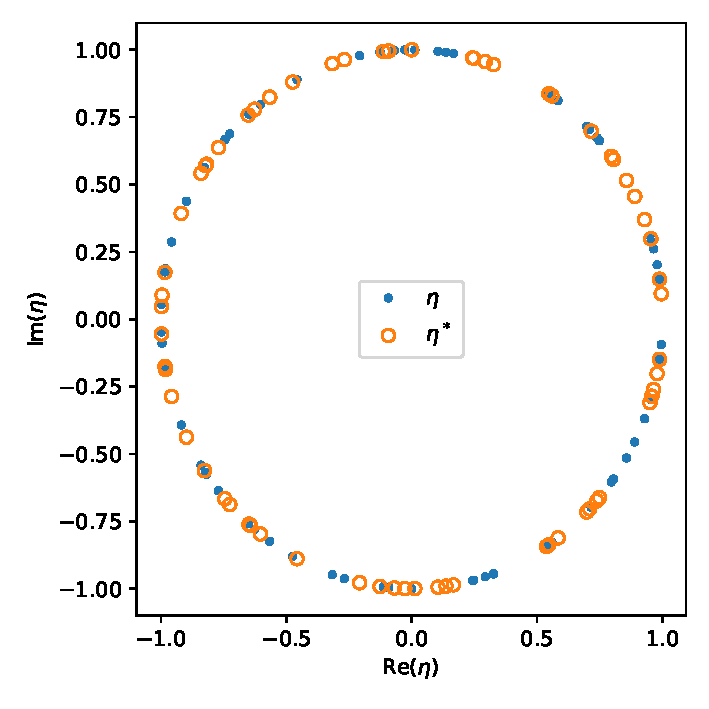
\includegraphics[width=0.46\textwidth]{../Plots/mbldtc_N=06_thetax=0.64pi_7f5eb9a5-72ff-4e83-9033-85285eac036c.pdf}}
  \subfigure[sample: bd6b58d5-66f6-4428-bb11-2cf64877a0b6]{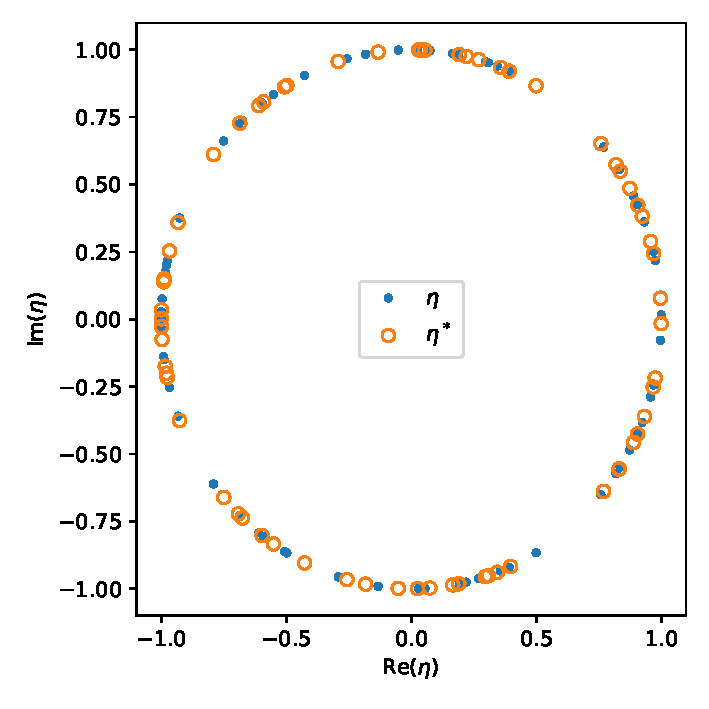
\includegraphics[width=0.46\textwidth]{../Plots/mbldtc_N=06_thetax=0.64pi_bd6b58d5-66f6-4428-bb11-2cf64877a0b6.pdf}}
    \caption{$N=6$, $\theta_x=0.64\pi$}
\end{figure}

\begin{figure}
  \centering
  \subfigure[sample: 8e67338c-f480-45a7-a8f0-a7e110499ba4]{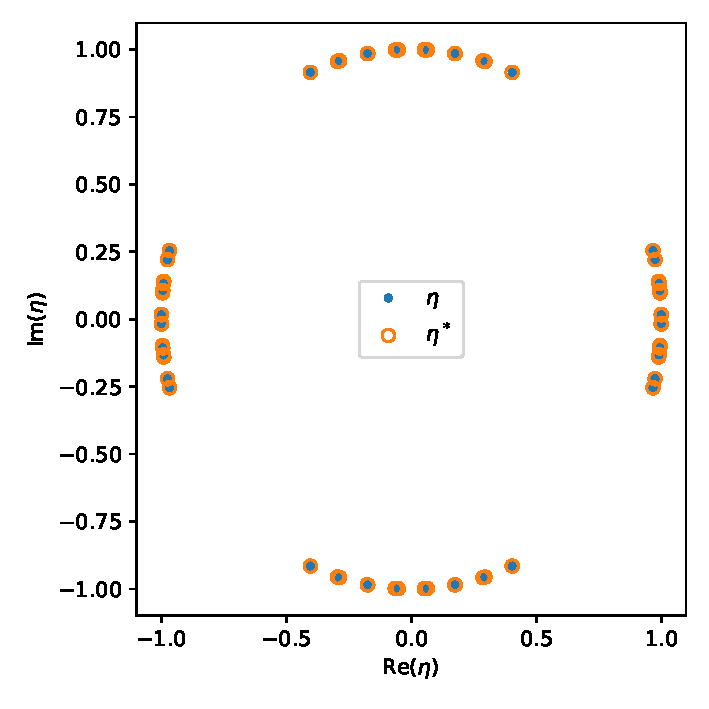
\includegraphics[width=0.46\textwidth]{../Plots/mbldtc_N=06_thetax=0.96pi_8e67338c-f480-45a7-a8f0-a7e110499ba4.pdf}}
  \subfigure[sample: db809334-cc72-4b15-b9ff-721dbd2a2afa]{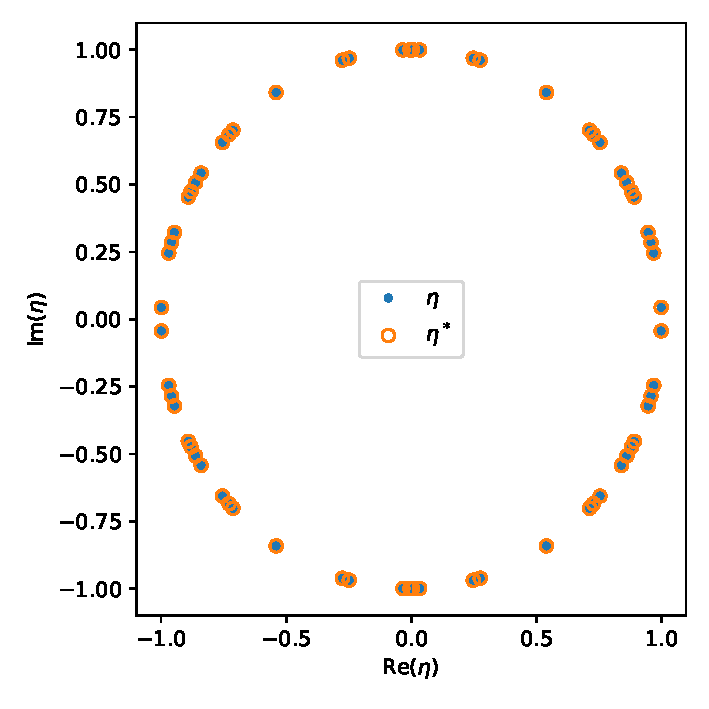
\includegraphics[width=0.46\textwidth]{../Plots/mbldtc_N=06_thetax=0.96pi_db809334-cc72-4b15-b9ff-721dbd2a2afa.pdf}}
  \caption{$N=6$, $\theta_x=0.96\pi$}
\end{figure}

\begin{figure}
  \centering
  \subfigure[sample: 228965e5-8f86-4b93-869c-5f6c7c77d39]{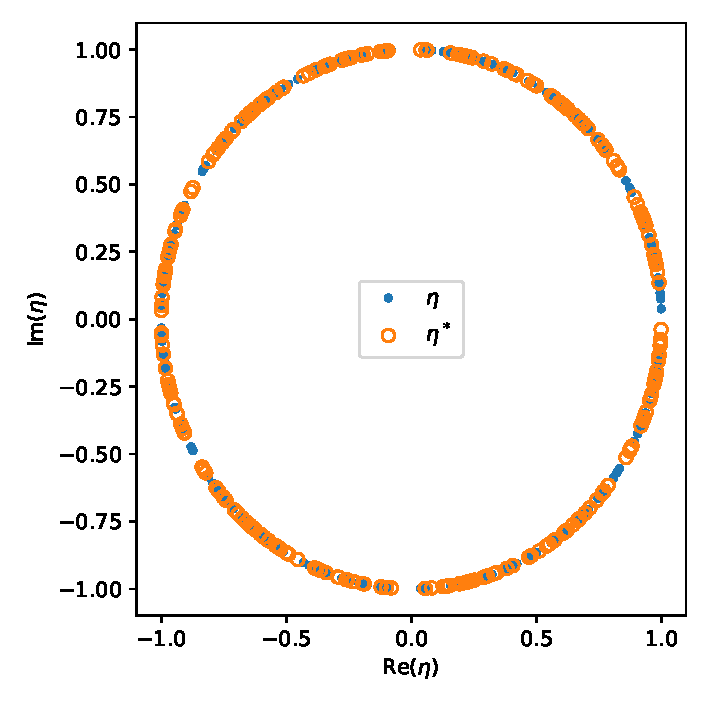
\includegraphics[width=0.46\textwidth]{../Plots/mbldtc_N=08_thetax=0.64pi_228965e5-8f86-4b93-869c-5f6c7c77d391.pdf}}
  \subfigure[sample: 886cc6c9-1e29-47d5-aa7b-71140c0f9a5d]{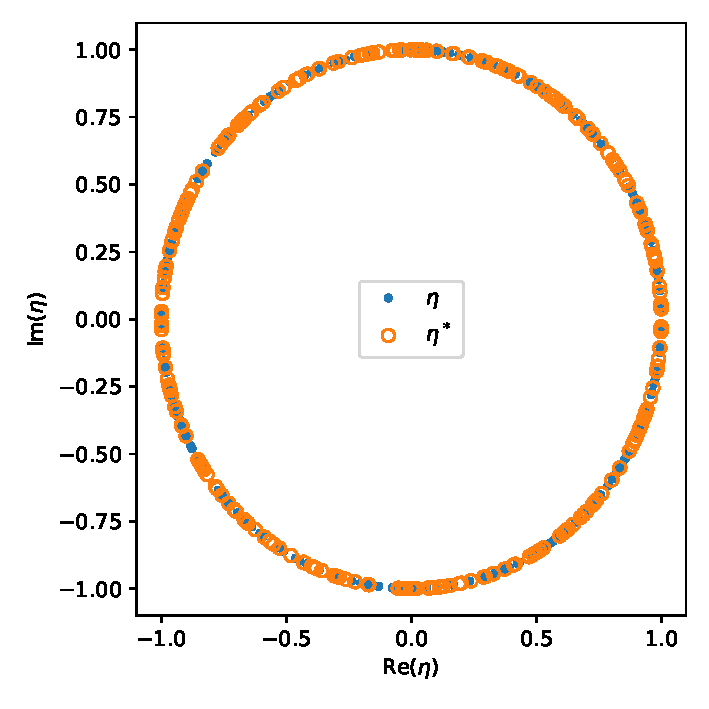
\includegraphics[width=0.46\textwidth]{../Plots/mbldtc_N=08_thetax=0.64pi_886cc6c9-1e29-47d5-aa7b-71140c0f9a5d.pdf}}
  \caption{$N=8$, $\theta_x=0.64\pi$}
\end{figure}

\begin{figure}
  \centering
  \subfigure[sample: e62ef79a-5af6-4da1-a889-6552643a5384]{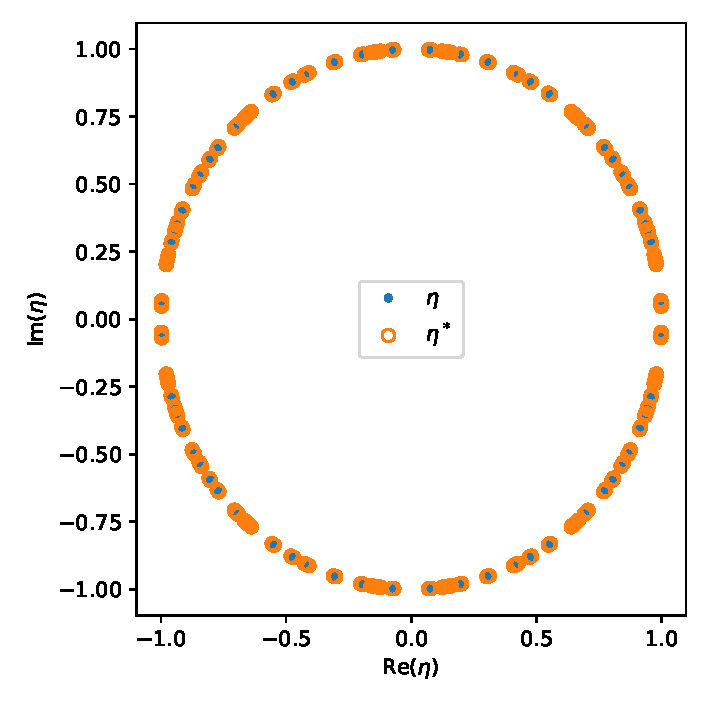
\includegraphics[width=0.46\textwidth]{../Plots/mbldtc_N=08_thetax=0.96pi_e62ef79a-5af6-4da1-a889-6552643a5384.pdf}}
  \subfigure[sample: f20ee949-20bd-456a-9edf-eccbbc1d4c03]{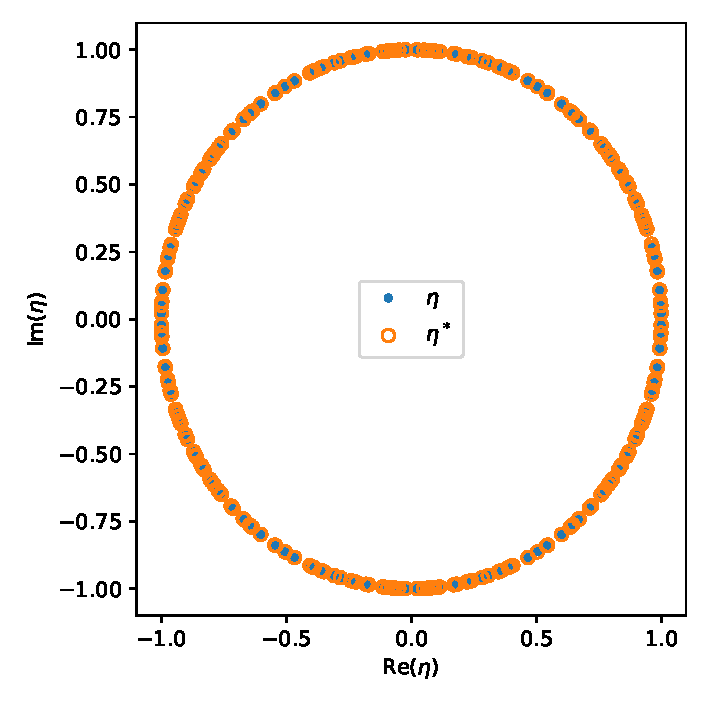
\includegraphics[width=0.46\textwidth]{../Plots/mbldtc_N=08_thetax=0.96pi_f20ee949-20bd-456a-9edf-eccbbc1d4c03.pdf}}
  \caption{$N=8$, $\theta_x=0.96\pi$}
\end{figure}

\begin{figure}
  \centering
  \subfigure[sample: 2a436997-d2e7-465d-8a66-522f4ad162af]{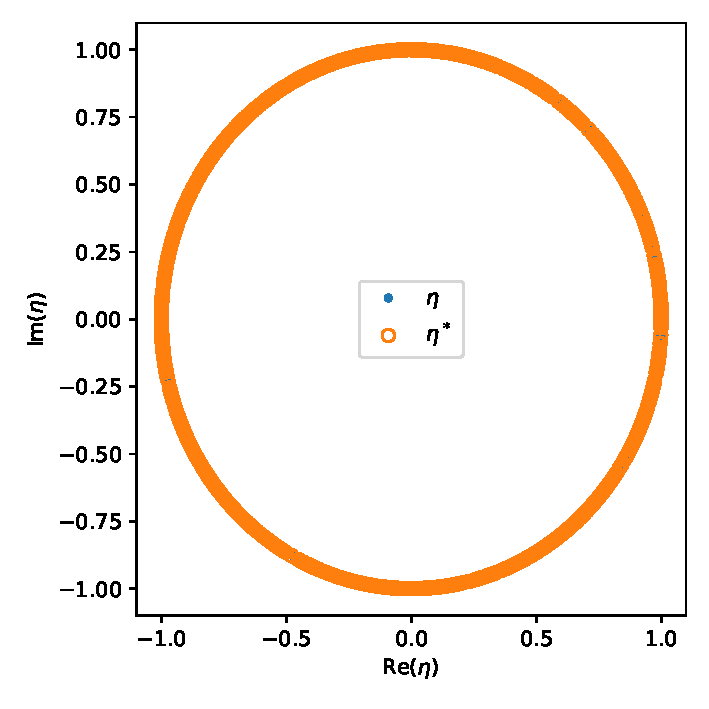
\includegraphics[width=0.46\textwidth]{../Plots/mbldtc_N=10_thetax=0.64pi_2a436997-d2e7-465d-8a66-522f4ad162af.pdf}}
  \subfigure[sample: fa3404ce-524f-4a9f-85c2-8315a6b19efb]{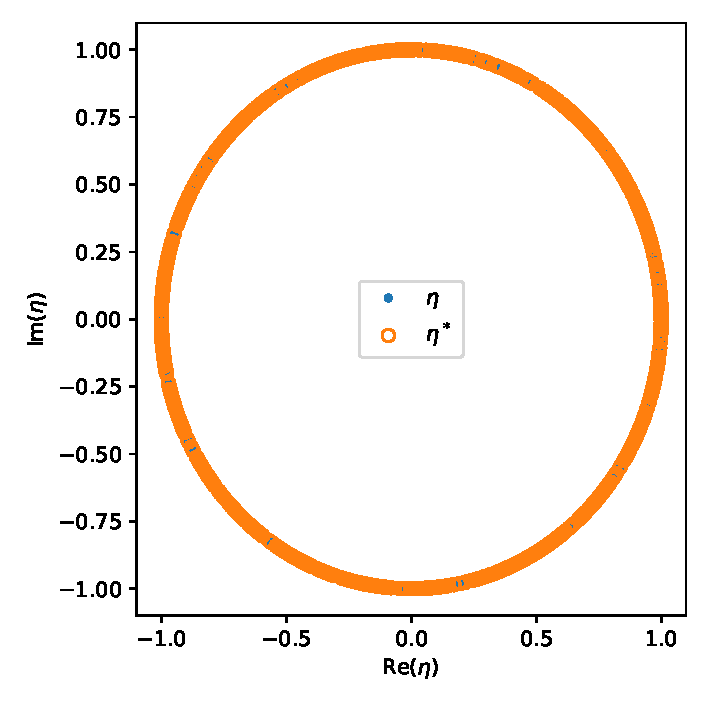
\includegraphics[width=0.46\textwidth]{../Plots/mbldtc_N=10_thetax=0.64pi_fa3404ce-524f-4a9f-85c2-8315a6b19efb.pdf}}
  \caption{$N=10$, $\theta_x=0.64\pi$}
\end{figure}


\begin{figure}
  \centering
  \subfigure[sample: 1366a22e-7e75-49e3-8dcf-96f76015aa14]{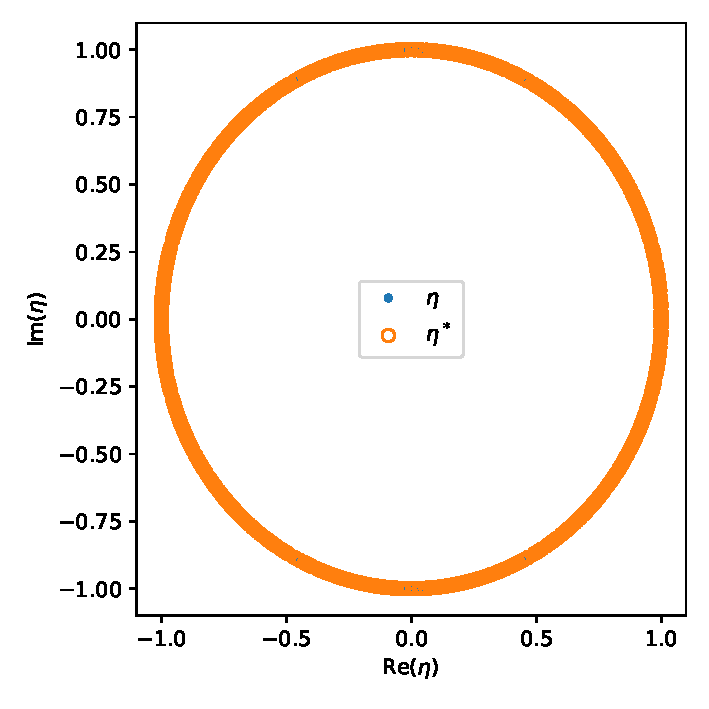
\includegraphics[width=0.46\textwidth]{../Plots/mbldtc_N=10_thetax=0.96pi_1366a22e-7e75-49e3-8dcf-96f76015aa14.pdf}}
  \subfigure[sample: d17e5ae9-1360-4254-b66e-7444d05b4a77]{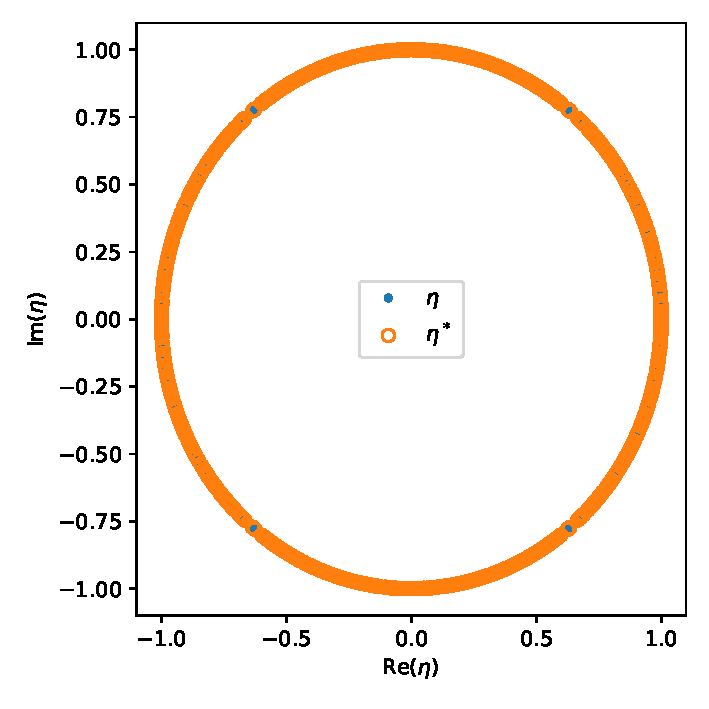
\includegraphics[width=0.46\textwidth]{../Plots/mbldtc_N=10_thetax=0.96pi_d17e5ae9-1360-4254-b66e-7444d05b4a77.pdf}}
  \caption{$N=10$, $\theta_x=0.96\pi$}
\end{figure}


\hypertarget{quantum-many-body-scars}{%
\section{Quantum many-body scars}\label{quantum-many-body-scars}}

Quantum many-body scars (QMBS) were discovered as an explanation for
periodic revivals of a Néel ordered initial state in a one-dimensional
array of neutral atoms with ground-to-Rydberg excitation
~\cite{bernien2017probing, bluvstein2021controlling}.

The Hamiltonian of this system in the basis of $| g \rangle$,
representing an atomic ground state and $| r \rangle$, representing an
atomic Rydberg state is effectively an Ising model with transverse and
longitudinal fields, which I call slanted field Ising
(SFI) model. For simplicity I consider the case of interactions onlu
between nearest neighbors when excited to atomic Rydberg states. In
the rotating frame at the angular frequency of the laser driving the
$| g \rangle \leftrightarrow | r \rangle$, transition and under the
rotating wave approximation, the Hamiltonian reads
\begin{equation}
    H_{\mathrm{SFI}}
    =
    \frac{\Omega}{2} \sum_{l} X_{l} -
    \frac{\Delta}{2} \sum_{l} Z_{l} +
    V_{rr} \sum_{l} \left( \frac{1 + Z_{l}}{2} \right)
                    \left( \frac{1 + Z_{l+1}}{2} \right),
\end{equation}
where $\Omega$ is the Rabi frequency for and $\Delta$ is the detuning
from the $| g \rangle \leftrightarrow | r \rangle$ transition and
$V_{rr}$ is the interaction between nearest-neighbor atoms when
excited to their Rydberg states.

A common regime of operation is the Rydberg blockade regime, which
occurs when $|V_{rr}| \gg \Omega$. In the nearest neighbor Rydberg
blockade and zero detuning $\Delta = 0$, regime, the system can be
described using a PXP model
~\cite{turner2018weak, turner2018quantum, maskara2021discrete},
whose Hamiltonian reads
\begin{equation}
    H_{\mathrm{PXP}} = \Omega \sum_{l} P_{l-1} X_{l} P_{l+1},
\end{equation}
where $P_{l}$ represents the projector onto the ground state,
$| g \rangle \langle g |$ for the $l$-th atom, hence the name `PXP'
model. The PXP model is known to have QMBS. Therefore, I expect QMBS
to be seen in the SFI model, in an appropriately constrained part of
the Hilbert space.

To study this I consider quantum quenches, but instead of looking at
the time evolution of an initial state, I consider the time evolution
operators
\begin{equation}
    U_{\mathrm{PXP}}(t) = \exp\left(-\im t H_{\mathrm{PXP}}\right),
\end{equation}
and
\begin{equation}
    U_{\mathrm{SFI}}(t) = \exp\left(-\im t H_{\mathrm{SFI}}\right),
\end{equation}
for the PXP and SFI models respectively. I plot the eigenvalues, $\eta$
of these time evolution operators and their complex conjugates $\eta^*$.
If there is eigenstate order involving pairing of eigenvalues, I expect
that every eigenvalue $\eta$ will be equal to one complex conjugate
$\eta^*$, as we saw for MBL-DTC.

I find that across different durations, \(t\) and system sizes \(N\),
the eigenvalues of \(U_{\mathrm{PXP}}(t)\) are complex conjugate
pairs, as I would expect for eigenstate
order. For \(U_{\mathrm{SFI}}(t)\), I find that fraction of the
eigenvalues of occur as complex conjugate pairs, perhaps being in the
constrained part of the Hilbert space.

\begin{figure}
  \centering
  \subfigure[SFI]{
    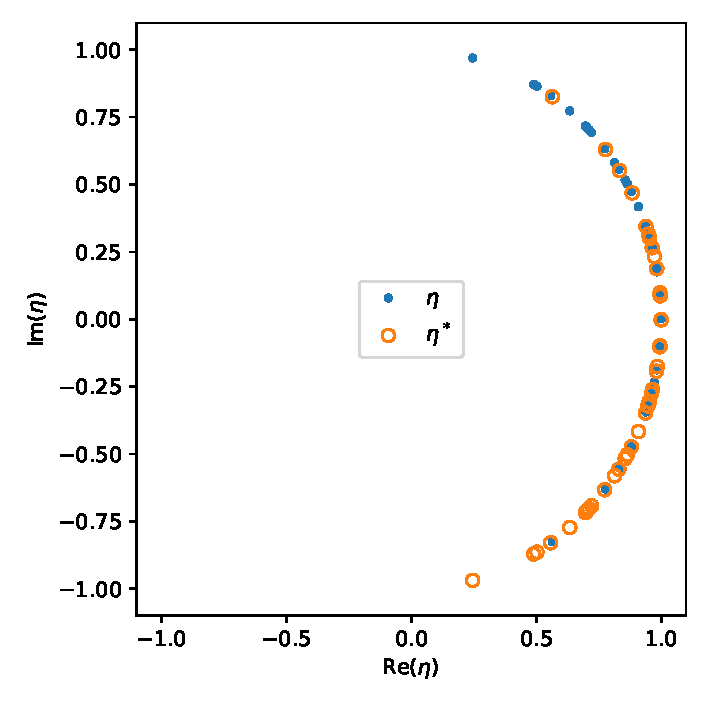
\includegraphics[width=0.44\textwidth]{../Plots/qmbs_sfim_N=06_tduration=0.5_Vrr=100_Omega=1.pdf}
  }
  \subfigure[PXP]{
    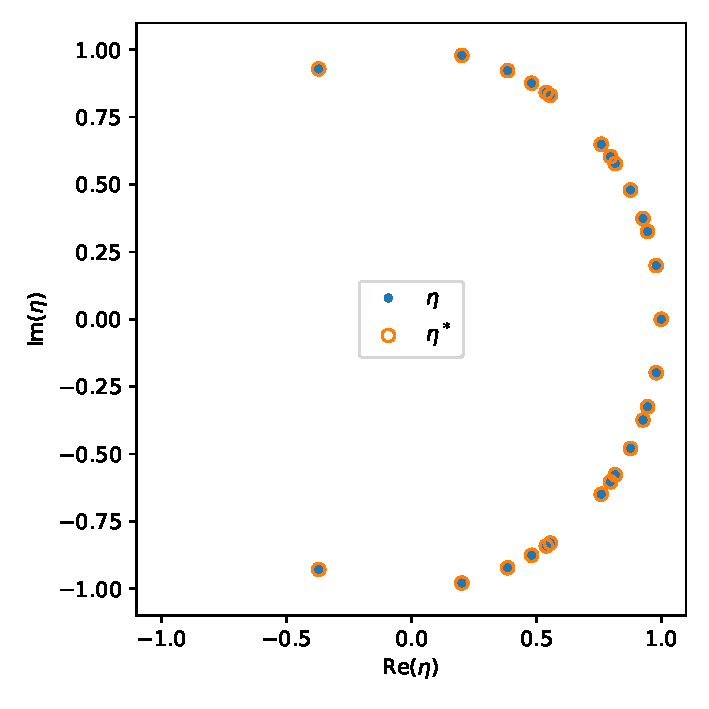
\includegraphics[width=0.44\textwidth]{../Plots/qmbs_pxp_N=06_tduration=0.5_Omega=1.pdf}
  }
  \caption{Eigenvalues, $\eta$ and their complex conjugates, $\eta^*$,
    of the the propagator, plotted in the complex place for $N=6$,
    $\Omega t=0.5$, for (a) SFI with $V_{rr}=100\Omega$ and (b) PXP
    Hamiltonians}
\end{figure}

\begin{figure}
  \centering
  \subfigure[SFI]{
    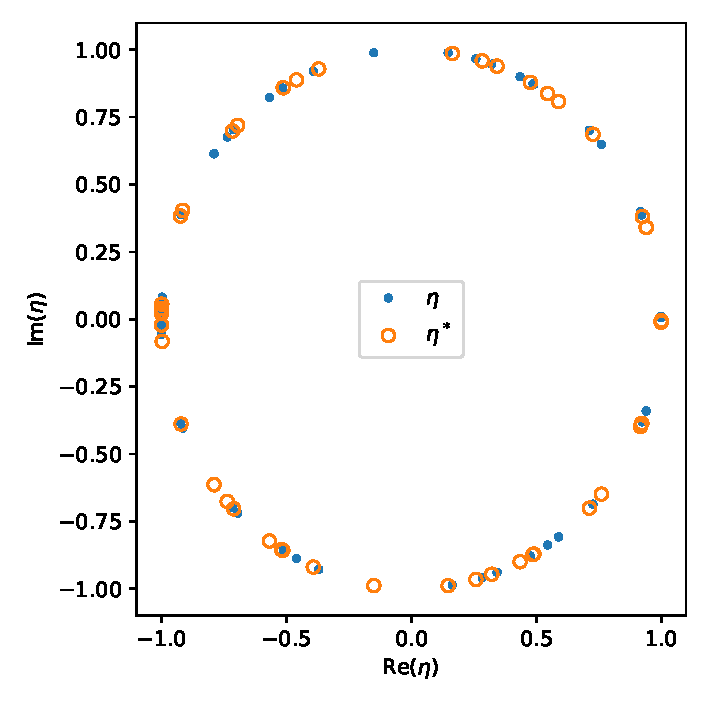
\includegraphics[width=0.44\textwidth]{../Plots/qmbs_sfim_N=06_tduration=2_Vrr=100_Omega=1.pdf}
  }
  \subfigure[PXP]{
    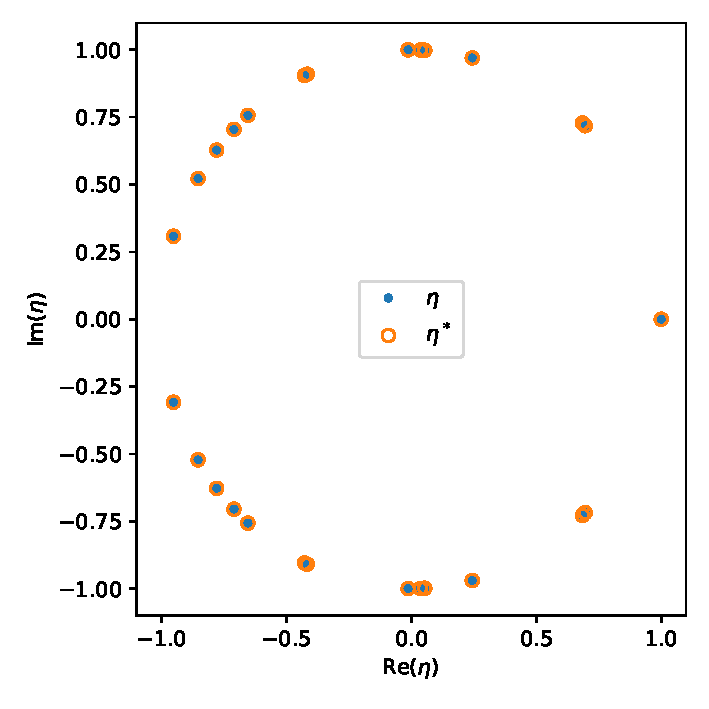
\includegraphics[width=0.44\textwidth]{../Plots/qmbs_pxp_N=06_tduration=2_Omega=1.pdf}
  }
  \caption{Eigenvalues, $\eta$ and their complex conjugates, $\eta^*$,
    of the the propagator, plotted in the complex place for $N=6$,
    $\Omega t=2$, for (a) SFI with $V_{rr}=100\Omega$ and (b) PXP
    Hamiltonians}
\end{figure}


\begin{figure}
  \centering
  \subfigure[SFI]{
    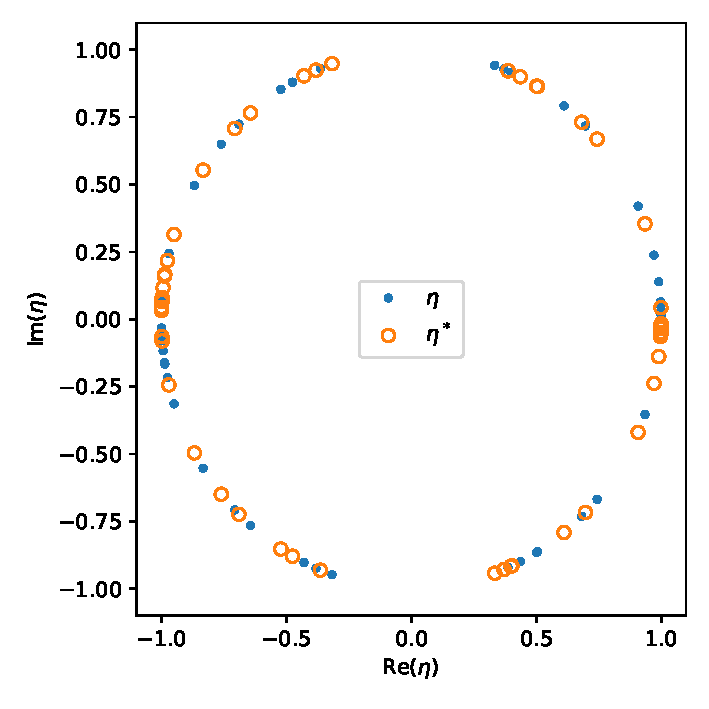
\includegraphics[width=0.44\textwidth]{../Plots/qmbs_sfim_N=06_tduration=6_Vrr=100_Omega=1.pdf}
  }
  \subfigure[PXP]{
    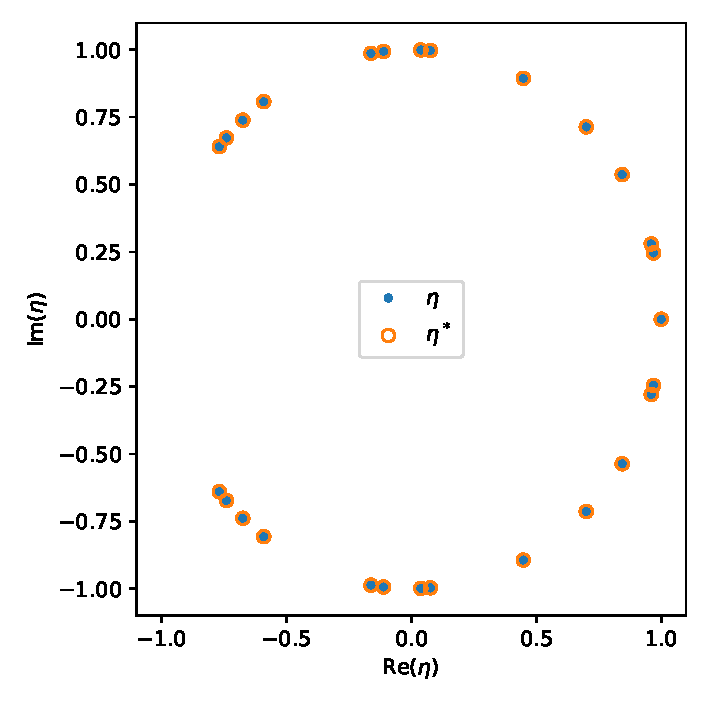
\includegraphics[width=0.44\textwidth]{../Plots/qmbs_pxp_N=06_tduration=6_Omega=1.pdf}
  }
  \caption{Eigenvalues, $\eta$ and their complex conjugates, $\eta^*$,
    of the the propagator, plotted in the complex place for $N=6$,
    $\Omega t=6$, for (a) SFI with $V_{rr}=100\Omega$ and (b) PXP
    Hamiltonians}
\end{figure}


\begin{figure}
  \centering
  \subfigure[SFI]{
    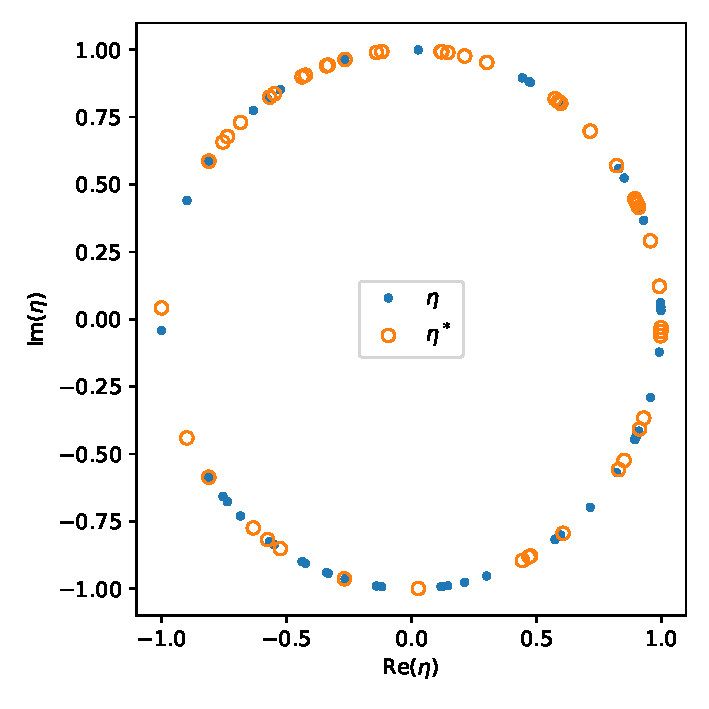
\includegraphics[width=0.44\textwidth]{../Plots/qmbs_sfim_N=06_tduration=11_Vrr=100_Omega=1.pdf}
  }
  \subfigure[PXP]{
    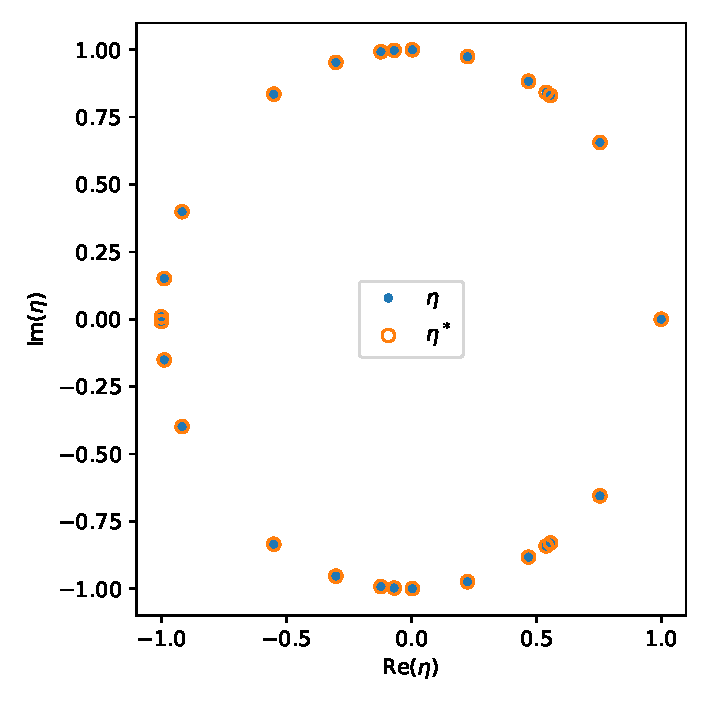
\includegraphics[width=0.44\textwidth]{../Plots/qmbs_pxp_N=06_tduration=11_Omega=1.pdf}
  }
  \caption{Eigenvalues, $\eta$ and their complex conjugates, $\eta^*$,
    of the the propagator, plotted in the complex place for $N=6$,
    $\Omega t=11$, for (a) SFI with $V_{rr}=100\Omega$ and (b) PXP
    Hamiltonians}
\end{figure}

%%%%%%%%%%%%%%%%

\begin{figure}
  \centering
  \subfigure[SFI]{
    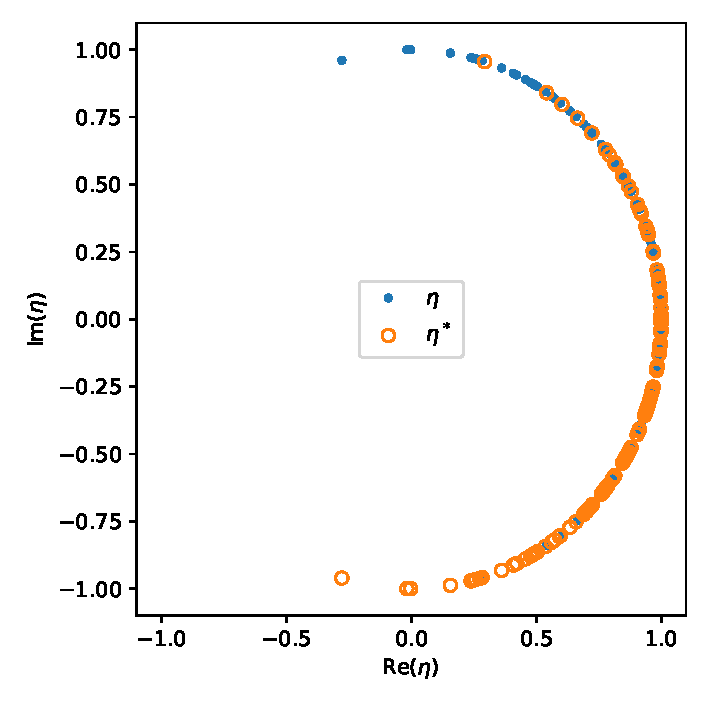
\includegraphics[width=0.44\textwidth]{../Plots/qmbs_sfim_N=08_tduration=0.5_Vrr=100_Omega=1.pdf}
  }
  \subfigure[PXP]{
    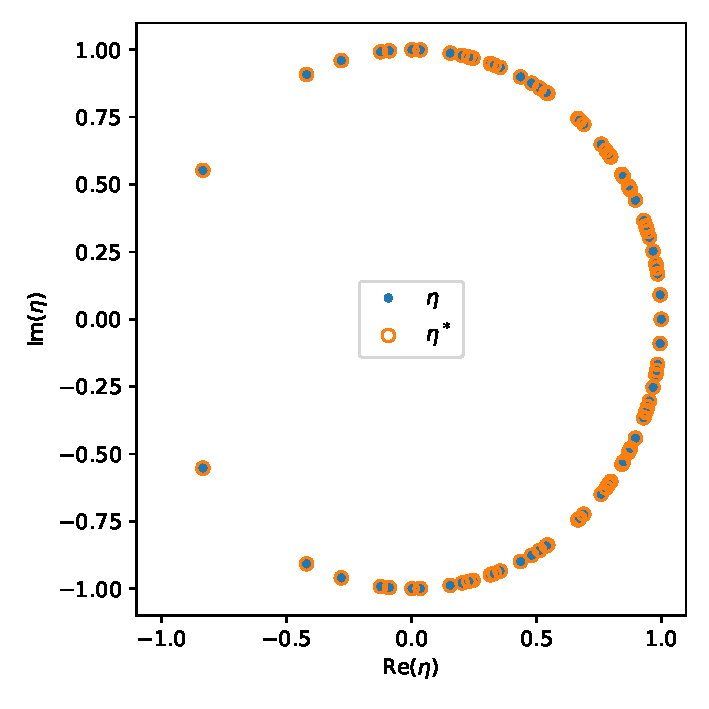
\includegraphics[width=0.44\textwidth]{../Plots/qmbs_pxp_N=08_tduration=0.5_Omega=1.pdf}
  }
  \caption{Eigenvalues, $\eta$ and their complex conjugates, $\eta^*$,
    of the the propagator, plotted in the complex place for $N=8$,
    $\Omega t=0.5$, for (a) SFI with $V_{rr}=100\Omega$ and (b) PXP
    Hamiltonians}
\end{figure}

\begin{figure}
  \centering
  \subfigure[SFI]{
    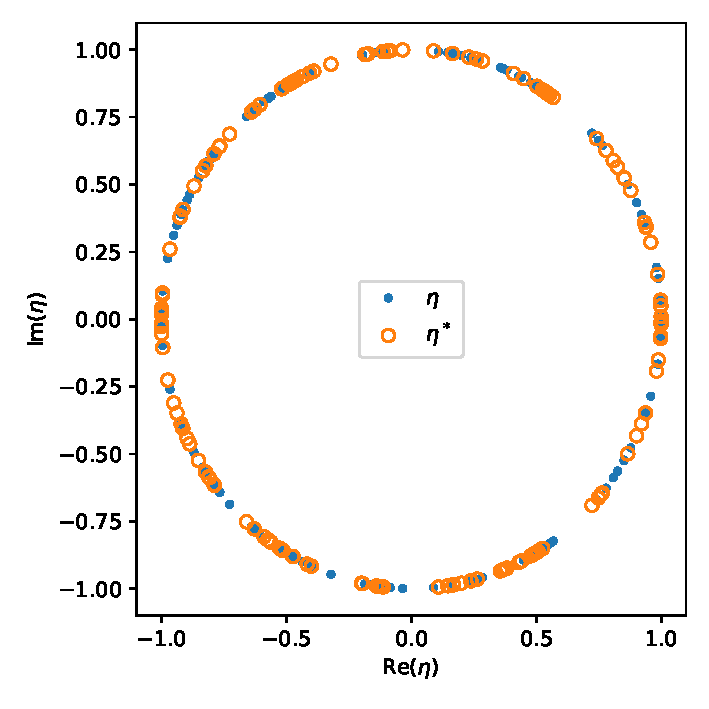
\includegraphics[width=0.44\textwidth]{../Plots/qmbs_sfim_N=08_tduration=2_Vrr=100_Omega=1.pdf}
  }
  \subfigure[PXP]{
    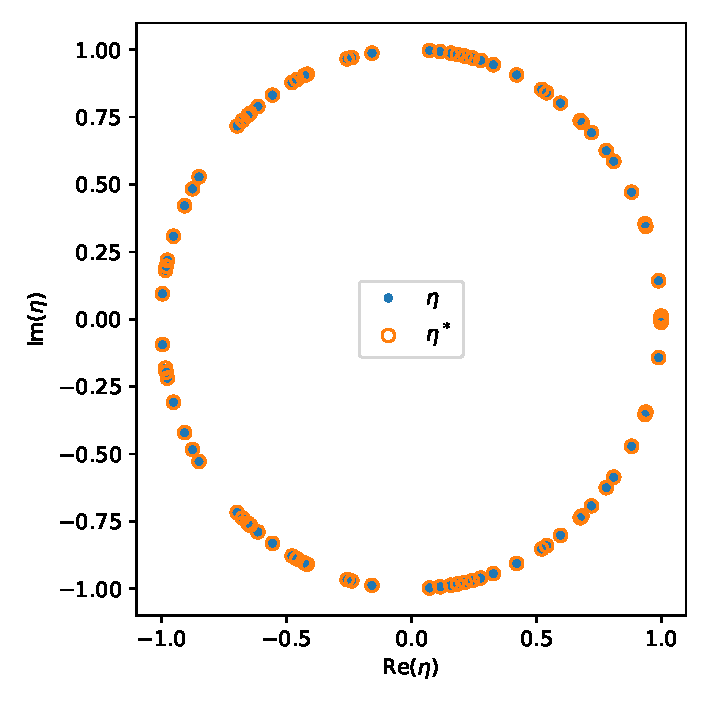
\includegraphics[width=0.44\textwidth]{../Plots/qmbs_pxp_N=08_tduration=2_Omega=1.pdf}
  }
  \caption{Eigenvalues, $\eta$ and their complex conjugates, $\eta^*$,
    of the the propagator, plotted in the complex place for $N=8$,
    $\Omega t=2$, for (a) SFI with $V_{rr}=100\Omega$ and (b) PXP
    Hamiltonians}
\end{figure}


\begin{figure}
  \centering
  \subfigure[SFI]{
    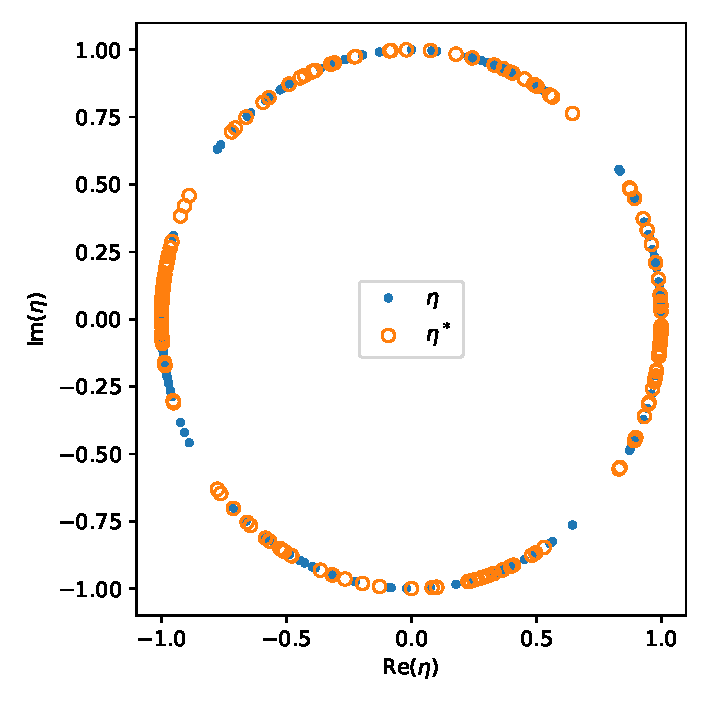
\includegraphics[width=0.44\textwidth]{../Plots/qmbs_sfim_N=08_tduration=6_Vrr=100_Omega=1.pdf}
  }
  \subfigure[PXP]{
    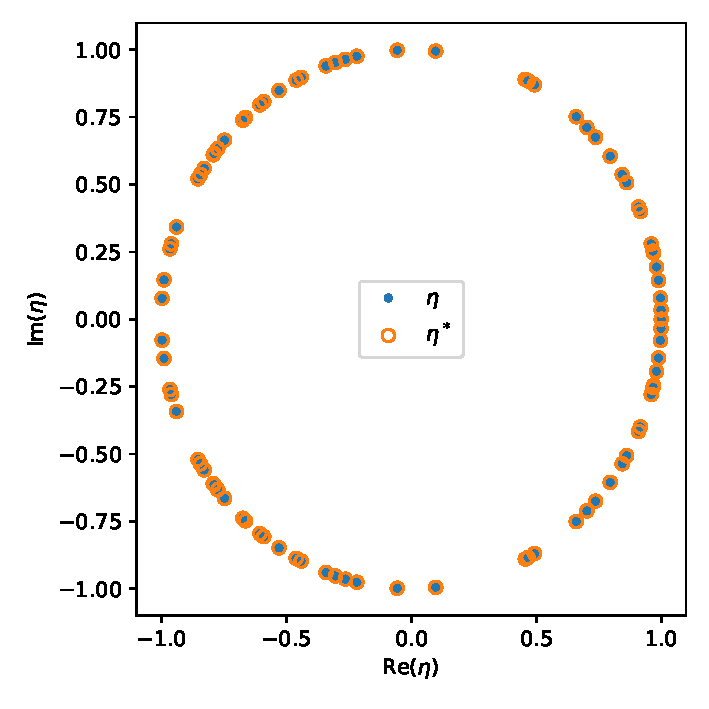
\includegraphics[width=0.44\textwidth]{../Plots/qmbs_pxp_N=08_tduration=6_Omega=1.pdf}
  }
  \caption{Eigenvalues, $\eta$ and their complex conjugates, $\eta^*$,
    of the the propagator, plotted in the complex place for $N=8$,
    $\Omega t=6$, for (a) SFI with $V_{rr}=100\Omega$ and (b) PXP
    Hamiltonians}
\end{figure}


\begin{figure}
  \centering
  \subfigure[SFI]{
    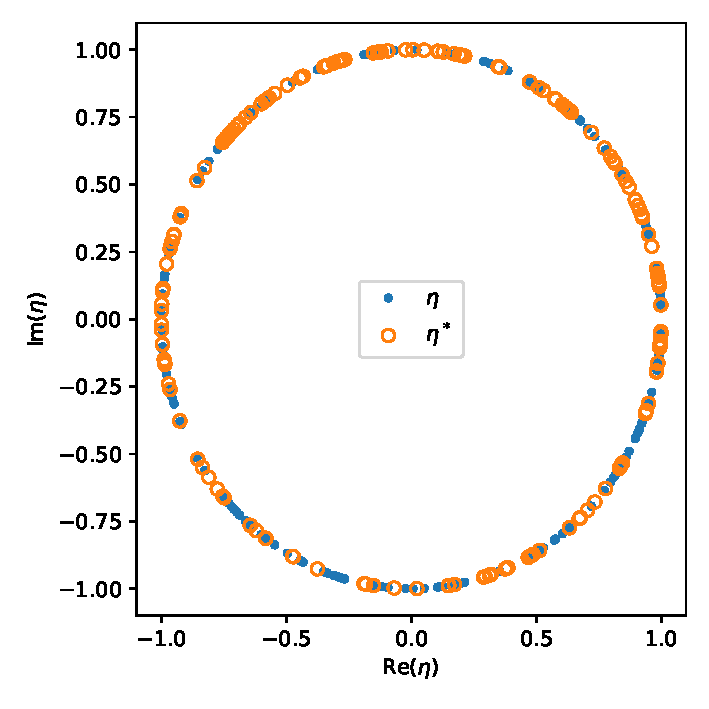
\includegraphics[width=0.44\textwidth]{../Plots/qmbs_sfim_N=08_tduration=11_Vrr=100_Omega=1.pdf}
  }
  \subfigure[PXP]{
    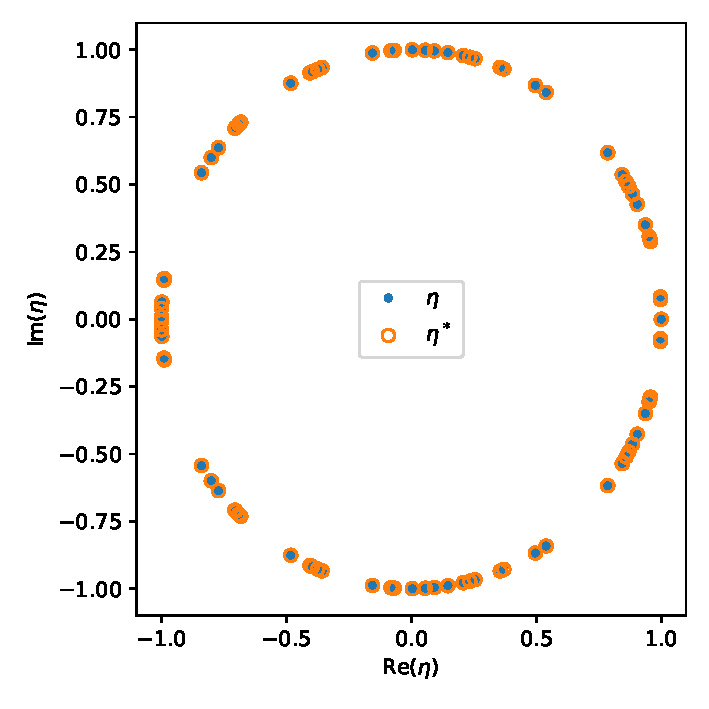
\includegraphics[width=0.44\textwidth]{../Plots/qmbs_pxp_N=08_tduration=11_Omega=1.pdf}
  }
  \caption{Eigenvalues, $\eta$ and their complex conjugates, $\eta^*$,
    of the the propagator, plotted in the complex place for $N=8$,
    $\Omega t=11$, for (a) SFI with $V_{rr}=100\Omega$ and (b) PXP
    Hamiltonians}
\end{figure}

%%%%%%%%%%%%%%%

\begin{figure}
  \centering
  \subfigure[SFI]{
    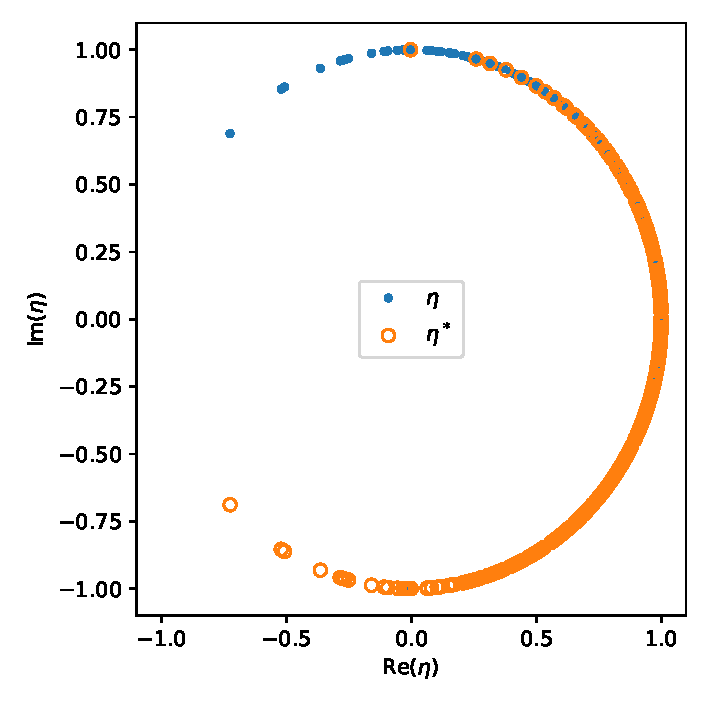
\includegraphics[width=0.44\textwidth]{../Plots/qmbs_sfim_N=10_tduration=0.5_Vrr=100_Omega=1.pdf}
  }
  \subfigure[PXP]{
    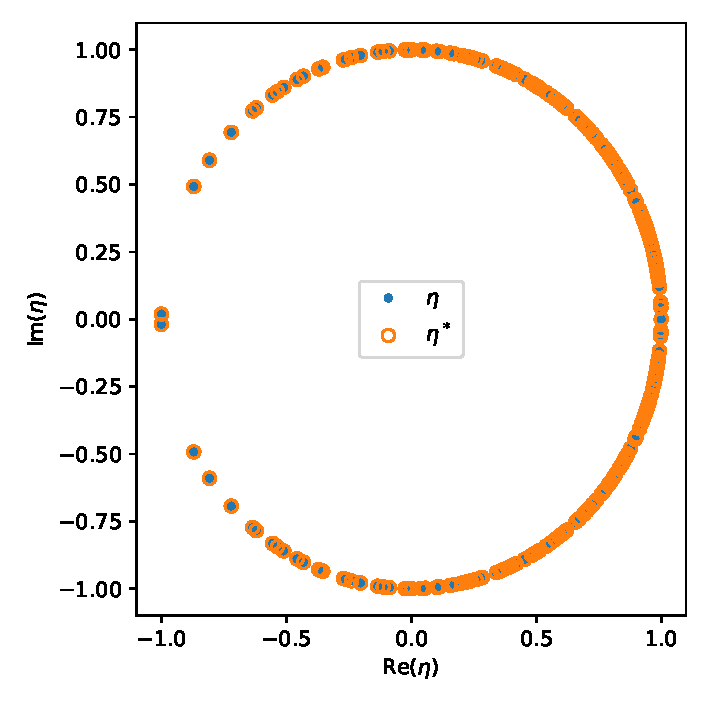
\includegraphics[width=0.44\textwidth]{../Plots/qmbs_pxp_N=10_tduration=0.5_Omega=1.pdf}
  }
  \caption{Eigenvalues, $\eta$ and their complex conjugates, $\eta^*$,
    of the the propagator, plotted in the complex place for $N=10$,
    $\Omega t=0.5$, for (a) SFI with $V_{rr}=100\Omega$ and (b) PXP
    Hamiltonians}
\end{figure}

\begin{figure}
  \centering
  \subfigure[SFI]{
    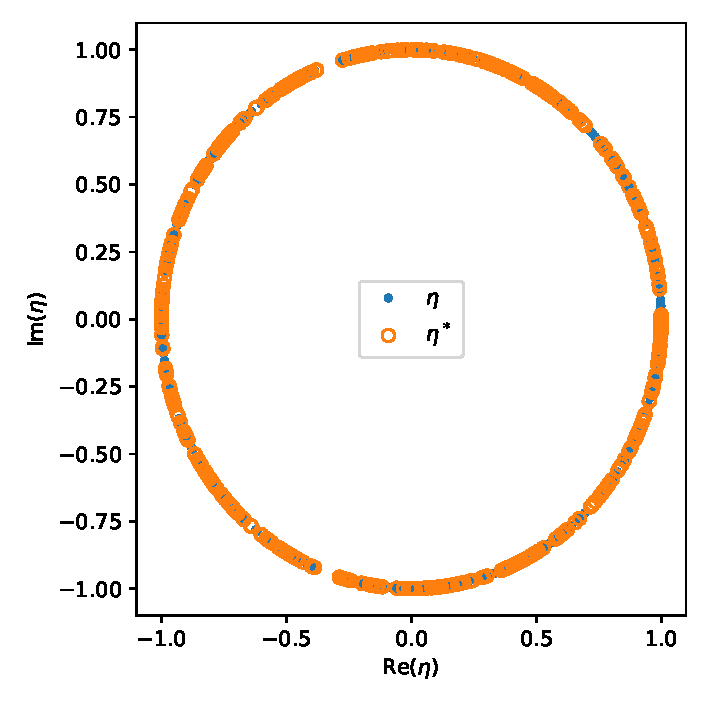
\includegraphics[width=0.44\textwidth]{../Plots/qmbs_sfim_N=10_tduration=2_Vrr=100_Omega=1.pdf}
  }
  \subfigure[PXP]{
    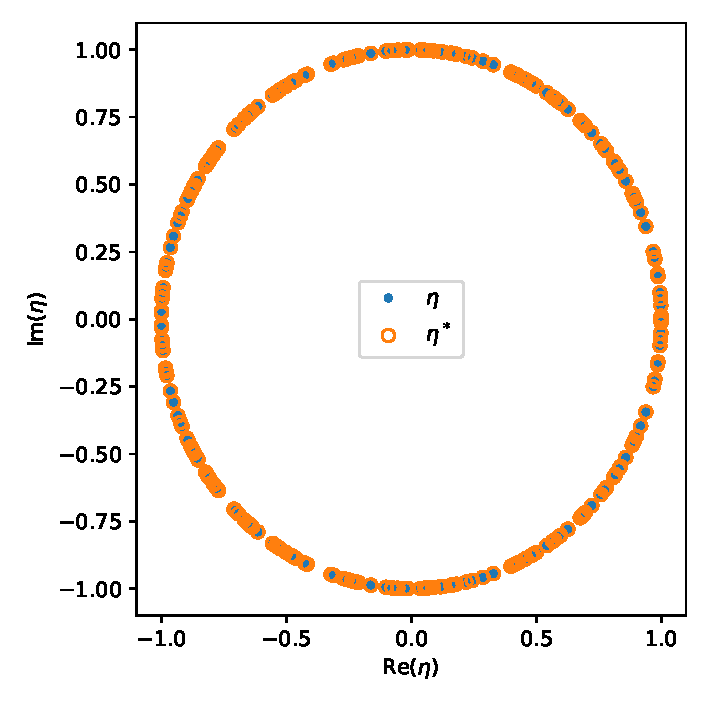
\includegraphics[width=0.44\textwidth]{../Plots/qmbs_pxp_N=10_tduration=2_Omega=1.pdf}
  }
  \caption{Eigenvalues, $\eta$ and their complex conjugates, $\eta^*$,
    of the the propagator, plotted in the complex place for $N=10$,
    $\Omega t=2$, for (a) SFI with $V_{rr}=100\Omega$ and (b) PXP
    Hamiltonians}
\end{figure}


\begin{figure}
  \centering
  \subfigure[SFI]{
    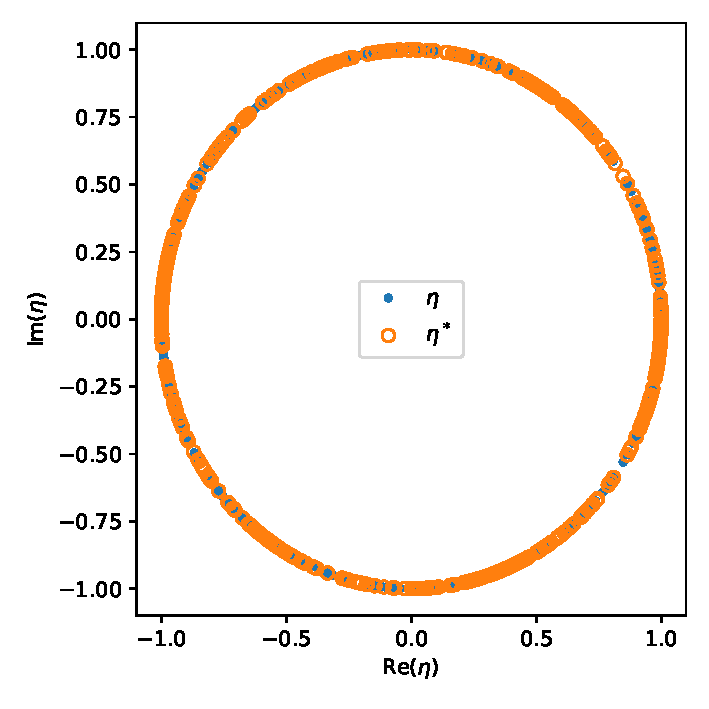
\includegraphics[width=0.44\textwidth]{../Plots/qmbs_sfim_N=10_tduration=6_Vrr=100_Omega=1.pdf}
  }
  \subfigure[PXP]{
    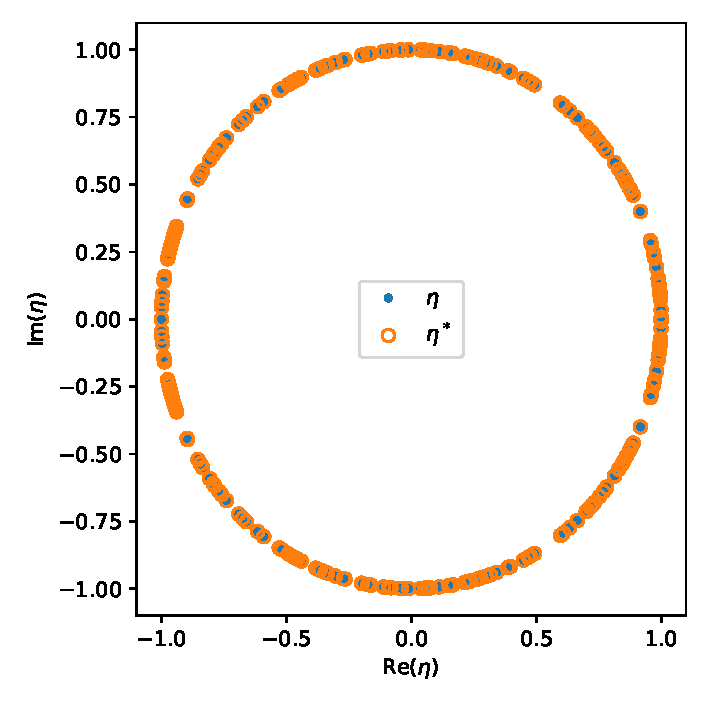
\includegraphics[width=0.44\textwidth]{../Plots/qmbs_pxp_N=10_tduration=6_Omega=1.pdf}
  }
  \caption{Eigenvalues, $\eta$ and their complex conjugates, $\eta^*$,
    of the the propagator, plotted in the complex place for $N=10$,
    $\Omega t=6$, for (a) SFI with $V_{rr}=100\Omega$ and (b) PXP
    Hamiltonians}
\end{figure}


\begin{figure}
  \centering
  \subfigure[SFI]{
    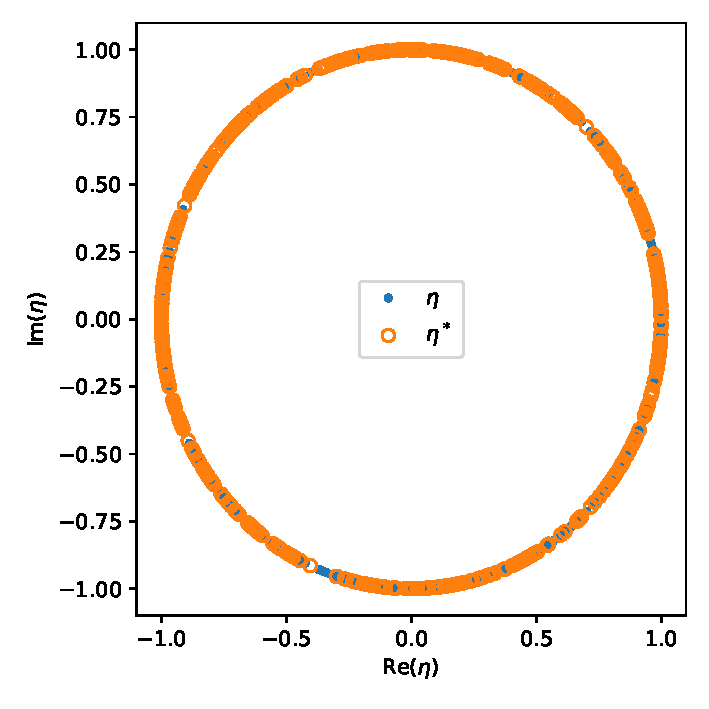
\includegraphics[width=0.44\textwidth]{../Plots/qmbs_sfim_N=10_tduration=11_Vrr=100_Omega=1.pdf}
  }
  \subfigure[PXP]{
    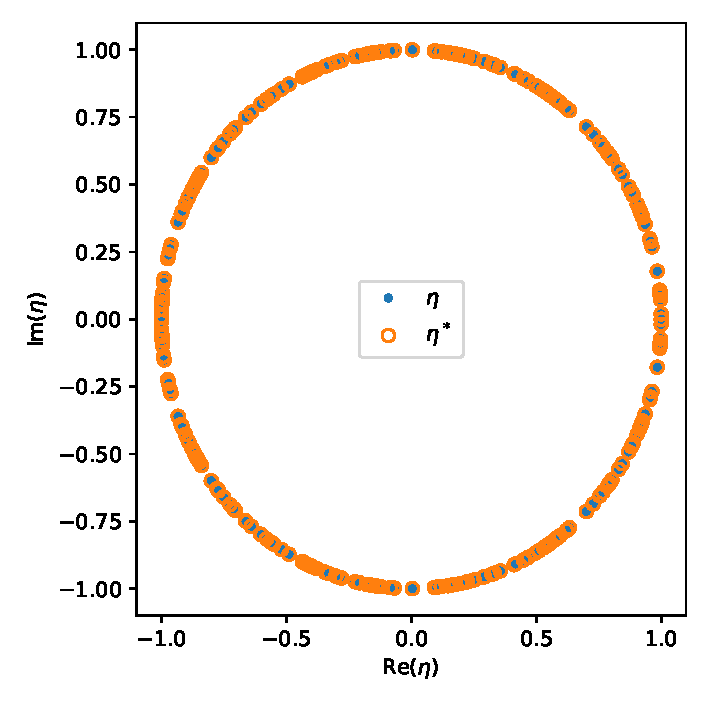
\includegraphics[width=0.44\textwidth]{../Plots/qmbs_pxp_N=10_tduration=11_Omega=1.pdf}
  }
  \caption{Eigenvalues, $\eta$ and their complex conjugates, $\eta^*$,
    of the the propagator, plotted in the complex place for $N=10$
    $\Omega t=11$, for (a) SFI with $V_{rr}=100\Omega$ and (b) PXP
    Hamiltonians}
\end{figure}


\bibliography{references}

\end{document}
